In \gls{mis}, as opposed to traditional open surgery, only small incisions are made in the patient's abdomen or pelvis in order to gain access to the area under surgery, hence causing less trauma beyond this confined area. This in general provides the patient with quicker recovery, shorter hospital stay and less scarring.
One type of \gls{mis} is \gls{laparoscopy}, invented in the beginning of the 20th century \citep{bib:laparoscopy}, where thin metal telescopes (laparoscopes) with specialized surgical tools attached are inserted into the patient through trocars, allowing the surgeon to maneuver the tools in the inflated abdomen guided by visual feedback from a flexible miniature camera (\gls{endoscope}) inserted alongside the surgical tools \citep{bib:fascrs}, see \autoref{fig:laparoscopy}.
In the 1980s robotic laparoscopic surgery was introduced as a master-slave system, where the surgeon controls a robot arm holding the surgical tools from a master console, instead of manipulating the instruments manually.

\vspace*{3mm}
\begin{figure}[htbp]
\centering
\begin{minipage}{0.39\textwidth}
\subbottom[Manual laparoscopic tools.]{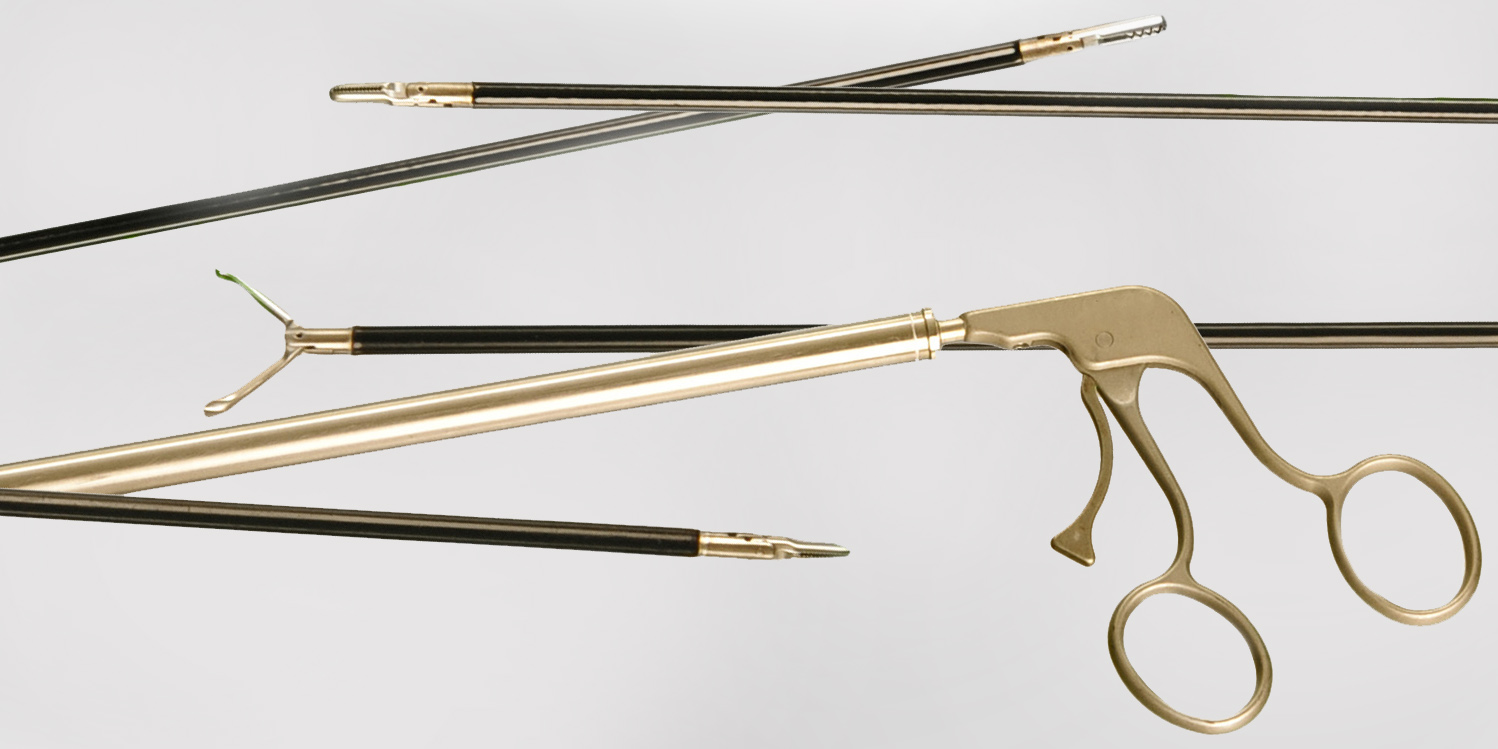
\includegraphics[width=\textwidth]{laparoscopic_instruments_manual_red.jpg}\label{fig:laparoscopic_instruments_manual}}%
\vspace*{3mm}
\subbottom[Robotic laparoscopic tools.]{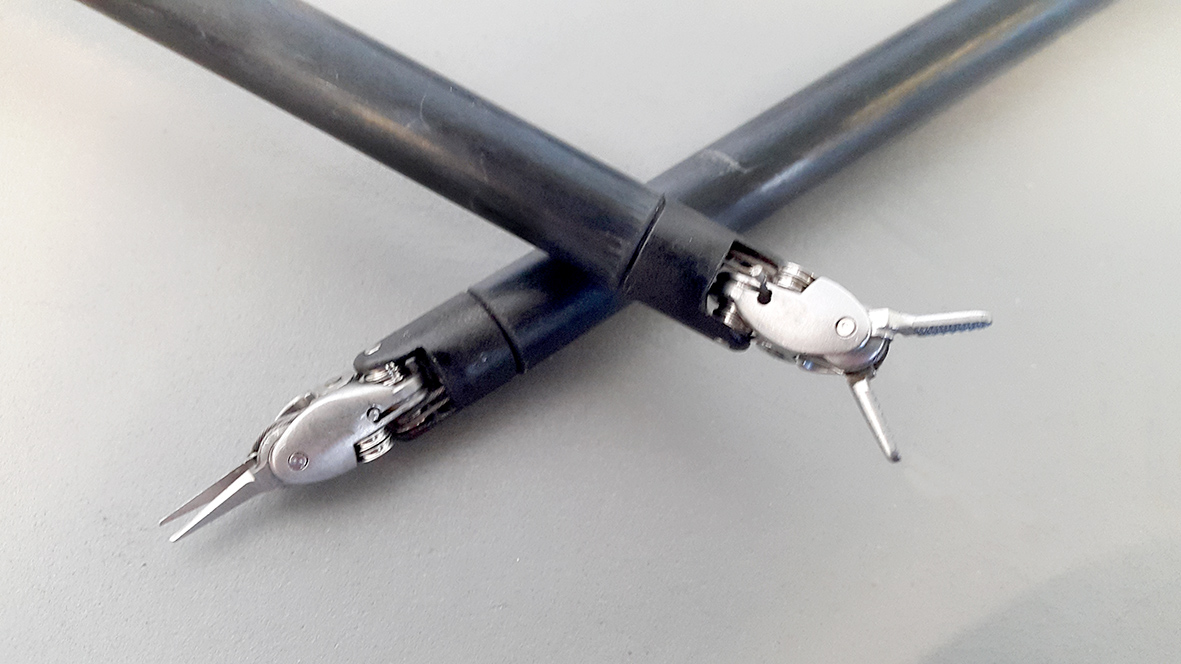
\includegraphics[width=\textwidth]{laparoscopy_20150312_134752.jpg}\label{fig:laparoscopy_20150312_134752}}%
\end{minipage}
\hspace*{5mm}
\begin{minipage}{0.258\textwidth}
\subbottom[Tool in trocar.]{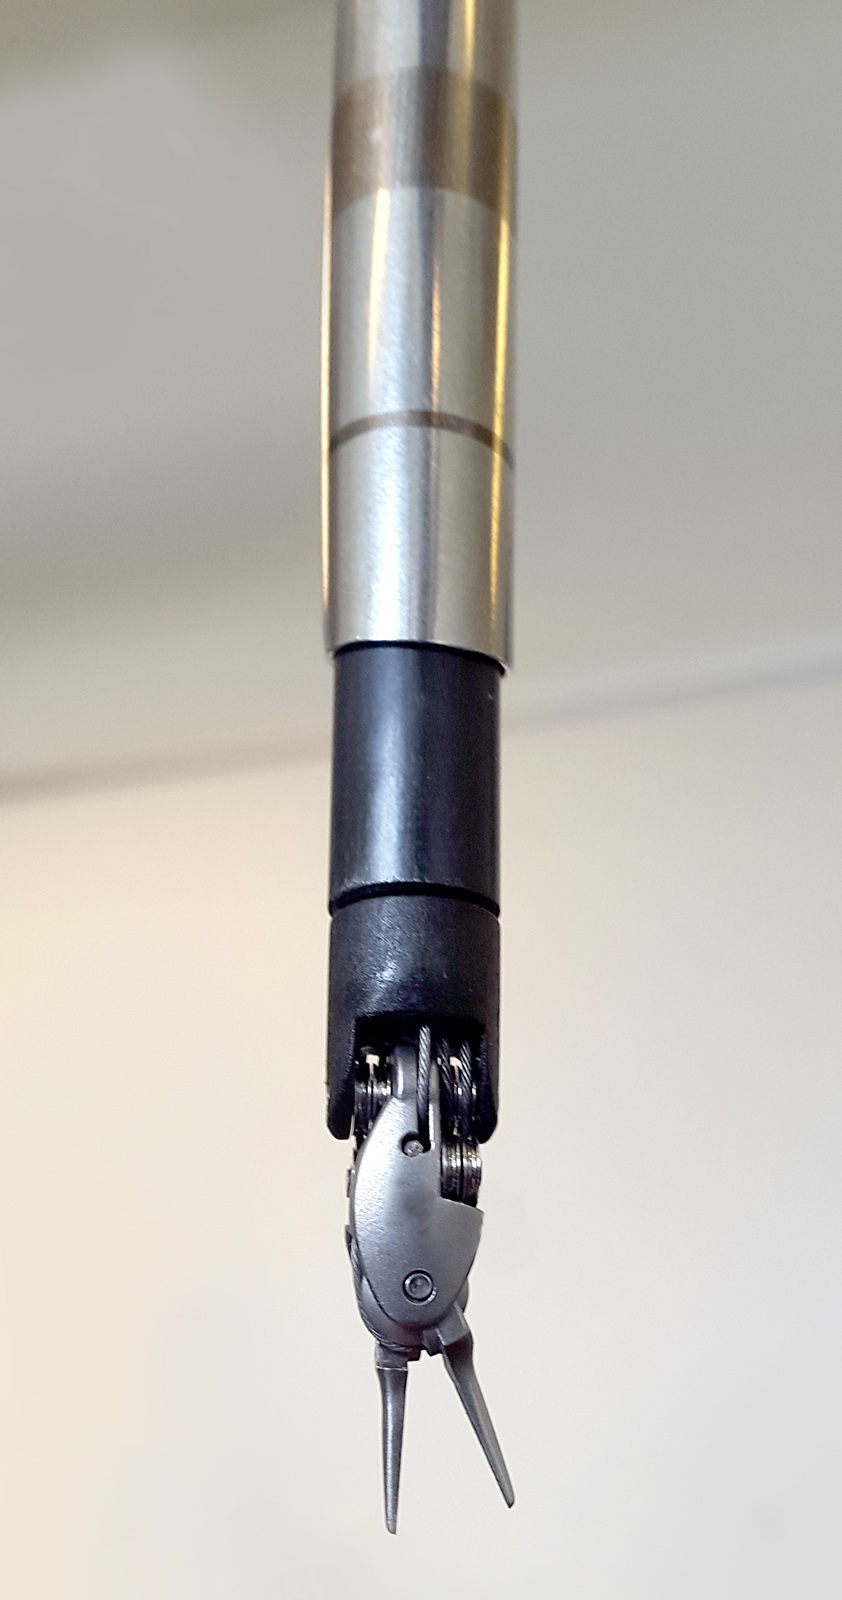
\includegraphics[width=\textwidth]{laparoscope_20150317_111908_red.jpg}\label{fig:laparoscope_20150317_111908}}%
\end{minipage}
\hspace*{5mm}
\begin{minipage}{0.258\textwidth}
\subbottom[Endoscope.]{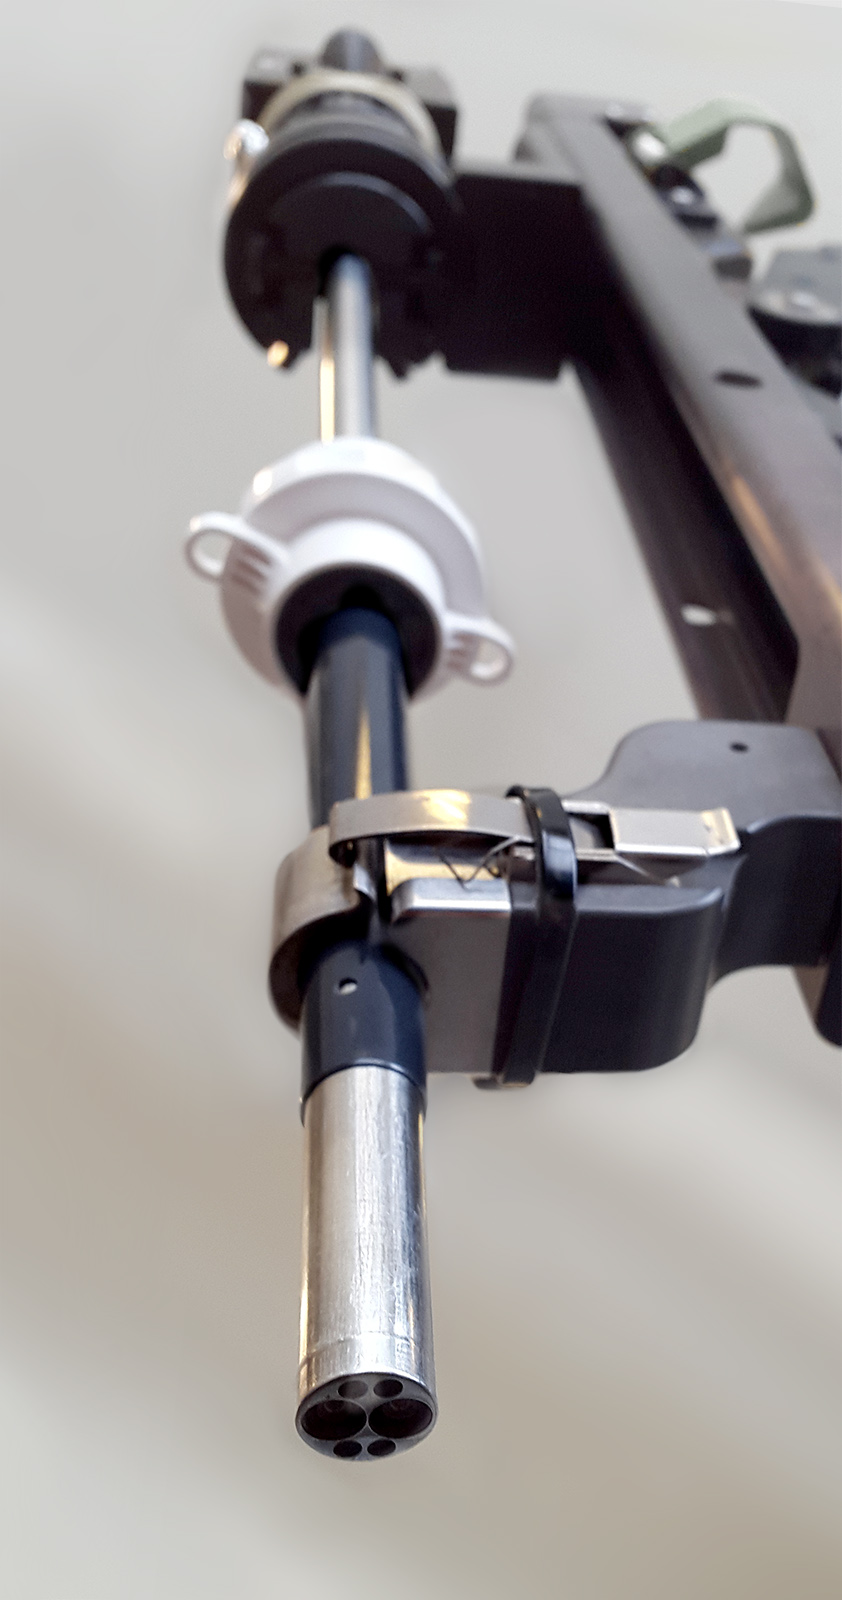
\includegraphics[width=\textwidth]{endoscope_20150430_124054.jpg}\label{fig:endoscope_20150430_124054}}%
\end{minipage}
\caption{Tools used in laparoscopic surgery.}
\label{fig:laparoscopy}
\end{figure}

\section{Highlights in the Development of Surgical Robotics}
While the idea of roboticized telemedicine dates back to 1925 \citep{bib:telemed_predict}, the development of telesurgery was founded by the \gls{nasa} in the 1970s %\citep{bib:telesurg_history} 
combining research within virtual reality, robotics and medicine, %\citep{bib:brown_univ}, 
and the first robotic surgery procedure was accomplished in 1985, %\citep{bib:telesurg_history}, 
followed by the first laparoscopic robotic surgical procedure in 1987 \citep{bib:telesurg_history,bib:brown_univ}.
In 1998 the first fully endoscopic robotic surgery and the initial beating-heart totally endoscopic coronary bypass procedure were performed \citep{bib:brown_univ}.


%The first commercially available surgical robot ROBODOC (from Curexo) was introduced and performed the first robotic joint replacement surgery in 1992, and in 1994 the AESOP (from Computer Motion) was the first robotic system approved by the \gls{fda} for general surgery \citep[p 74]{bib:telesurg_history,bib:surgical_book}.

The first commercially available surgical robot was introduced in the early 1990. At the same time major research within telesurgery was funded by \gls{darpa}, %and two main teleoperation systems were developed from this research: da Vinci (from Intuitive Surgical) and Zeus (from Computer Motion) \citep{bib:telesurg_history}.
concurrent with the U.S. Army developing the \gls{mash} for loading and teleoperating wounded soldiers in vehicular operating rooms \citep{bib:telesurg_history,bib:brown_univ}.

%In the early 1990s the U.S. Army developed \gls{mash} for loading and teleoperating wounded soldiers in vehicular operating rooms \citep{bib:brown_univ}, and in 1993 the idea for a robotic slave manipulator arm was conceived by Madhani after watching an episode of the tv-show M*A*S*H [SurgRob], and he created the Black Falcon during his work at MIT \citep{bib:black_falcon} later becoming he prototype of the da Vinci arms.

Surgical robots teleoperated from more than a few meters away is, however, still incipient. In 1996 the first tests were performed demonstrating the successful use of telementoring and telemanipulation of the endoscope by a surgeon placed several 100 m away from the operating room, % \citep{bib:telesurg_history}. 
%In the late 1990s \gls{nasa} and \gls{darpa} sponsored research within light-weight and deployable space surgical robotics for remote teleoperation, resulting in two main robotic systems: the Raven (from University of Washington) and M7 (from SRI International) [SurgRob].
%
%and in 2000 da Vinci (from Intuitive Surgical) became the first robotic surgical system  to be approved by the \gls{fda} for general laparoscopic surgery \citep{bib:mddi}.
%
and in 2001 the first transatlantic telesurgical procedure, the Lindbergh Operation, was performed by a team of French doctors in New York %manipulating the arms of a Zeus robot to perform a gall bladder 
operating on a patient in Strasbourg \citep{bib:telesurg_history}. More research into remotely telementored and teleoperated robotic surgery was performed during the 2000s with the \gls{neemo} projects  %in the Aquarius undersea lab in Florida %, in 2003 with Zeus controlled from Ontario 2500 km away \citep[pp 75, 81]{bib:surgical_book} and in 2006 and 2007 with Raven and M7 controlled from Seattle \citep[pp 28, 82]{bib:surgical_book}. 
%
and as part of the \gls{darpa} Trauma Pod program launched in 2005 \citep{bib:surgical_book,bib:docatadist}.

%In 2005 \gls{darpa} launched the Trauma Pod program for developing an unmanned autonomous and semi-autonomous mobile military operation platform, funding research for e.g. SRI and for the Raven project. The goal of the first phase of the project was achieved in 2007 with the successful demonstration of a prototype trauma pod consisting of a da Vinci robot, a \gls{mash} stretcher and a custom nurse robot \citep[p 30]{bib:surgical_book}. The second phase aims at miniaturizing and integrating the systems \citep[p 31]{bib:surgical_book}, and in 2005 a demonstration was performed by roboticists, surgeons, aerospace engineers and networking experts in the desert placing the Raven patient manipulator and the controller console 100 m apart and relaying the communication link via a drone \citep{bib:docatadist}.



%In 2006 the first-ever demonstration of unmanned telesurgery with M7 [SurgRob]
%
%M7 performed the world's first automated ultrasound guided tumor biopsy in 2007 [SurgRob]
%
%2008 neuroArm was first used to remove a brain tumor [SurgRob]

%\gls{nasa}'s first experiment in a zero gravity environment was performed with an acceleration compensated M7 in 2007 on a parabolic flight \citep[pp 29, 76, 85]{bib:surgical_book}, and in 2011 \gls{nasa} sent the humanoid robot Robonaut 2 to \gls{iss}, and it has since been trained in telemedicine [SurgRob].







\section{State-of-the-Art in Surgical Robotics}
Most surgical robots used for telesurgery are master-slave systems which can be fully controlled by the surgeon, see \autoref{fig:master-slave_surgery}. % \citep{bib:raven_debride}. 
The patient manipulator consists of 2-4 robotic arms, each having 6-7 \gls{dof} % \citep{bib:raven_debride} 
including the arm, wrist and the end-effector (the laparoscopic tool), one of the arms holding a stereo-vision \gls{endoscope} \citep{bib:raven_debride}. 
The end-effectors are positioned by high-precision motors and are able to reach spaces a human hand cannot \citep{bib:docatadist}, and furthermore development is progressing within flexible end-effector tools \citep[p 74]{bib:surgical_book}. %, but even microrobots entering the body through natural orifices and controlled via electromagnetic fields or nanosensors and -actuators are being developed [SurgRob].

\begin{figure}[htbp]
\hspace*{-5mm}
\subbottom[Surgeon master console and slave robotic patient manipulator.]{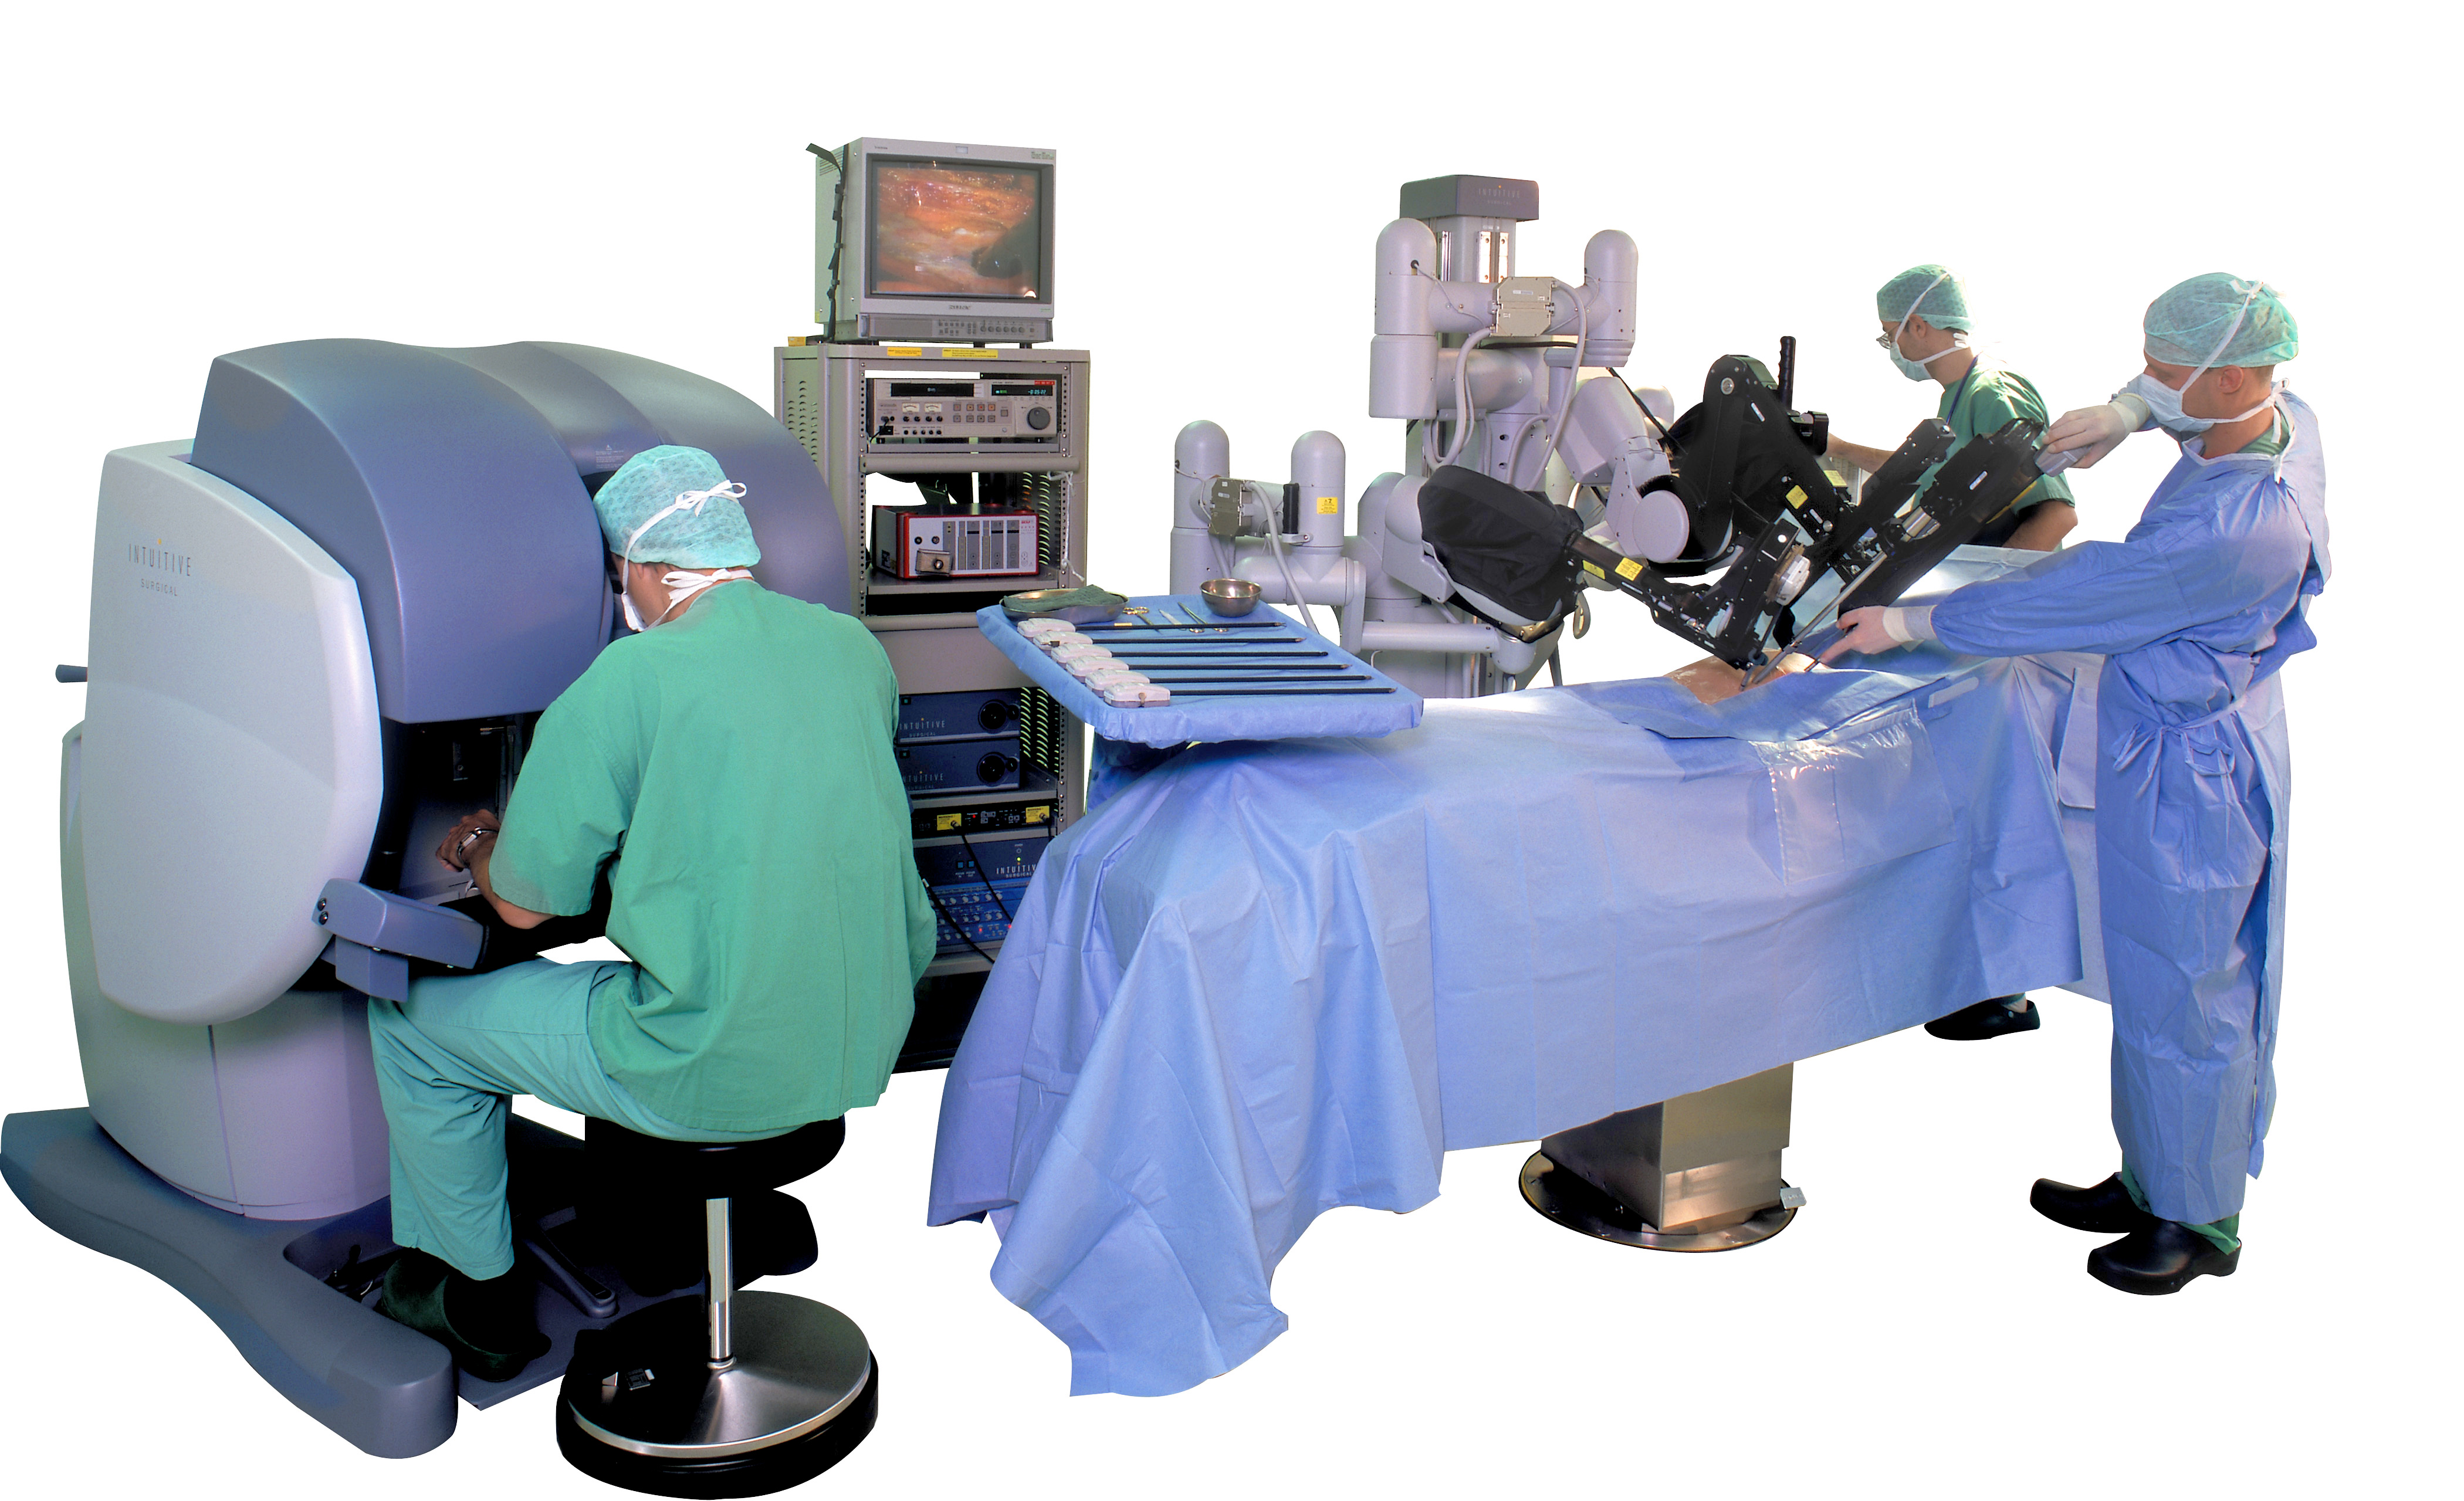
\includegraphics[width=0.5\pdfpagewidth]{davinci_surgical_system.jpg}\label{fig:davinci_surgical_system}}%
\subbottom[The robotic patient manipulator.]{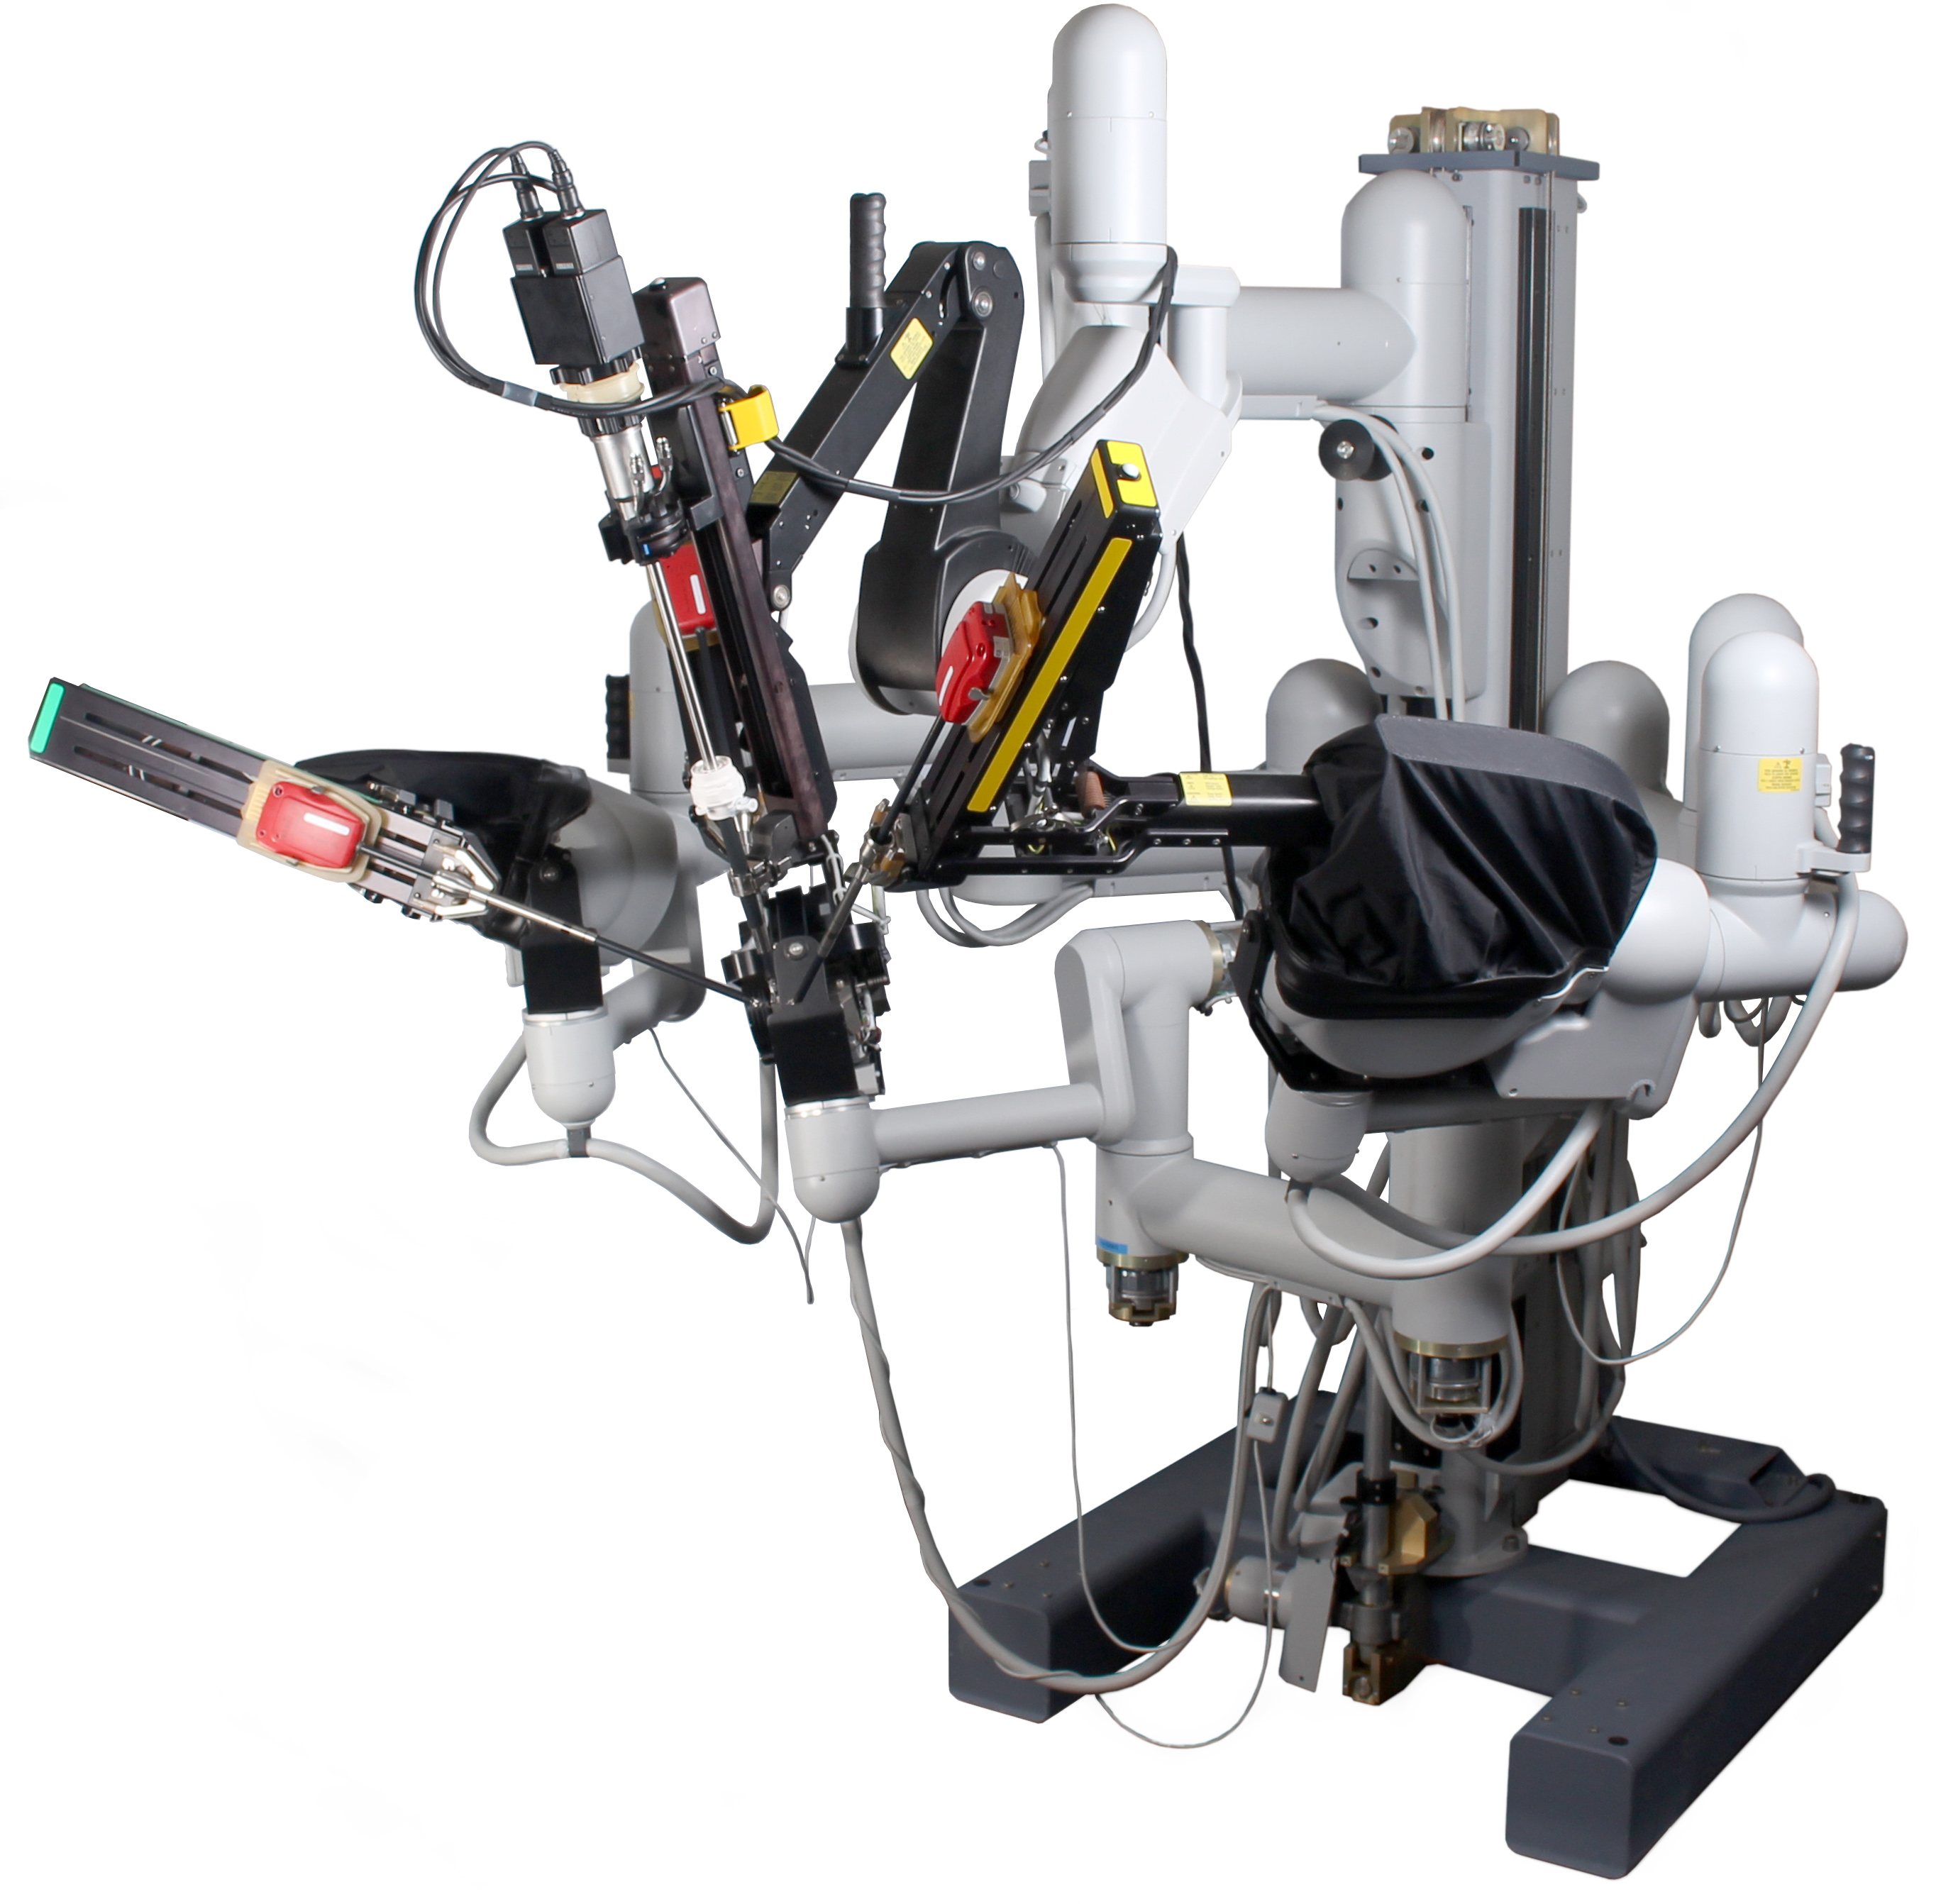
\includegraphics[width=0.4\textwidth]{robot_base_frame1.jpg}\label{fig:robot_base_frame}}%
\caption{Example of a master-slave robotic surgical system: the da Vinci.}
\label{fig:master-slave_surgery}
\end{figure}

The 3D visual feedback from the endoscope is sent to the master console, % which can have eye-tracking for adaptive field of view and safety stop if the surgeon's gaze is not fixed at the operation site [SurgRob]. The 
and the control signals for the surgical instrument are generated with the controller joystick, which scales the surgeon's movements down to micro-movements \citep{bib:intuitive_monopoly} steerable through the (zoomed) 3D visual feedback. It also filters away tremor, and development is made within haptic feedback to the joystick \citep[p 89]{bib:surgical_book}, enhancing the surgeon's feel, enabling greater dexterity, accuracy and stability than a human hand.

In the first generations of surgical robotics the master and slave had to be in the same room, %(as is the case with da Vinci) \citep{bib:telesurg_history,bib:raven_debride,bib:surgical_book},
but although the feasibility of conducting surgical interventions remotely has been demonstrated, there has not been drivers strong enough to justify its implementation \citep[p 38]{bib:surgical_book}. Experiments and development are made within minimizing and coping with delays for long-distance telesurgery and within miniaturization and robustness of the surgical robotic systems for use in harsh environments such as war and space. %, e.g. for da Vinci's potentially closest competitor, the open-source Raven.

Robotic surgical procedures are beginning to show superiority to conventional surgery for some procedures, but is still considerably more expensive \citep{bib:docatadist}. 
%In some cases robotic procedures are faster than conventional surgeon procedures [SurgRob], but still in other it is much slower \citep{bib:raven_ii,bib:raven_debride}.
Autonomous procedures are still only implemented for entirely pre-planned motions of an operation, and depending on the type of operation not all subtasks in an operation are suited for autonomy \citep{bib:raven_debride,bib:raven_ii}.


%\textcolor{red}{New generation: surgical care not only to soldiers but also to remote locations lacking specialized physicians. - better tactile feedback because the surgeon needs to feel the tissue and the difference in its stiffness}


 
%\subsection{The da Vinci Surgical System}
%Although several \gls{fda} approved robotic surgical systems exist, da Vinci is still the only commercially available system \citep{bib:docatadist,bib:intuitive_monopoly}. 
%The first da Vinci prototype was developed at SRI under contract with the U.S. Army in the late 1980s \citep{bib:mddi,bib:brown_univ}, and in the early 1990s \gls{darpa} invested in the research \citep[p 74]{bib:surgical_book}. In % the mid 1990s SRI licensed the manipulator design of Madhani along with many other patents, and in 
%1995 SRI founded Intuitive Surgical and the focus shifted from battlefield to commercial use in hospitals \citep{bib:intuitive_monopoly}.
%In 1997 the first human trials were performed \citep{bib:intuitive_monopoly} %, in 1999 the first market-ready da Vinci began tests [SurgRob] 
%and the system was first approved by the FDA in 2000 \citep{bib:intuitive_monopoly,bib:brown_univ}. From 2000 until the merger in 2003 Intuitive Surgical and Computer Motion had a number of lengthy patent litigations \citep{bib:intuitive_monopoly,bib:telesurg_history}.





%The da Vinci Surgical System still has the predominant market share with more than 3000 units installed worldwide due to being the first-mover in the field and due to their many patents \citep{bib:intuitive_monopoly}, and has only had one serious case of a patient dying after surgery (2002) [SurgRob].
%The expiration of their patents in 2015 and 2016 \citep{bib:intuitive_monopoly} shows promise of many other robotic surgery systems entering the market, as both American, Canadian, European and not least Asian similar systems exist that are considerably cheaper than the da Vinci, and also more lightweight.

%In 2013 Intuitive released the da Vinci Research Kit platform, built from mechanical components from first generation da Vinci (two arms and a surgeon console), open-source electronics and university-developed software \citep{bib:raven_observ}.

%\subsection{The Raven Surgical Robot}
%One potential challenger to da Vinci is the Raven \cite{bib:mddi}, an light-weight open-architecture 2-armed surgical robot \citep{bib:raven_debride,bib:raven_ii} originally developed by University of Washington funded by multiple U.S. government agencies including the Army and the \gls{dod} \citep[p 27]{bib:surgical_book}.
%Raven-II is installed at 10 different universities in the U.S. and one in France \citep{bib:raven_ii}, sharing research innovations and using open-source software (including the ROS middleware) to create surgery subtasks \citep{bib:raven_debride}. 
%As Intuitive Surgical's patents gradually expire the University of Washington is considering the possibility of spinning off the Raven into a start-up company \citep{bib:economist}.
%
%The Raven robot is focused on remote telesurgery (with notable latency) in harsh conditions \citep{bib:docatadist}, and research at University of California has been made in teaching a computer model to autonomously mimic laparoscopic surgeons from recordings dynamic and kinematic data of their motions in a multi-state statistical Hidden Markov Model \citep{bib:economist}. 
%The primary difficulty reported from controlling the Raven has been state estimation, necessary because of the uncertainty inherent in actuators and encoders connected to flexible elements via long cables \citep{bib:raven_debride} and the necessity of collision avoidance of the arms.
